\documentclass{article}

\usepackage{amsmath}
\usepackage{booktabs}
\usepackage[a4paper,textwidth=14cm, top=1cm, bottom=1cm,includehead,includefoot,
centering,footskip=1.5cm]{geometry}
\usepackage{graphicx}
\usepackage{hyperref}
% \usepackage{mathtools}
\usepackage{natbib}
\bibliographystyle{plainnat}

\hypersetup{
  colorlinks=true,
  linkcolor=blue,
  citecolor=blue,
  filecolor=blue,
  urlcolor=blue
}

\title{A New Model-Based Notion of Variable Importance}
\date{}
\author{Author 1\\ Author 1 address \and Author 2\\Author 2 address}

\begin{document}

\maketitle


%%%%%%%%%%%%%%%%%%%%%%%%%%%%%%%%%%%%%%%%%%%%%%%%%%%%%%%%%%%%%%%%%%%%%%%%%%%%%%%%
% Abstract
%%%%%%%%%%%%%%%%%%%%%%%%%%%%%%%%%%%%%%%%%%%%%%%%%%%%%%%%%%%%%%%%%%%%%%%%%%%%%%%%
\begin{abstract}
Keep to 200 words or less and don't use references or mathematical markup.
\end{abstract}


%%%%%%%%%%%%%%%%%%%%%%%%%%%%%%%%%%%%%%%%%%%%%%%%%%%%%%%%%%%%%%%%%%%%%%%%%%%%%%%%
% Introduction
%%%%%%%%%%%%%%%%%%%%%%%%%%%%%%%%%%%%%%%%%%%%%%%%%%%%%%%%%%%%%%%%%%%%%%%%%%%%%%%%
\section{Introduction}

Talk about the improtance of extracting information from black-box models, blah, blah, blah.


\subsection{Partial dependence plots}

\citet{harrison-1978-hedonic} were among the first to analyze the well-known Boston housing data. One of their goals was to find a housing value equation using data on median home values from $n = 506$ census tracts in the suburbs of Boston from the 1970 census; see \citet[Table IV]{harrison-1978-hedonic} for a description of each variable. The data violate many classical assumptions like linearity, normality, and constant variance. Nonetheless, \citeauthor{harrison-1978-hedonic}---using a combination of transformations, significance testing, and grid searches---were able to find a reasonable fitting model ($R^2 = 0.81$). Part of the payoff for there time and efforts was an interpretable prediction equation which is reproduced in Equation~\eqref{eqn:boston}.
\begin{equation}
\label{eqn:boston}
\begin{aligned}
\widehat{\log\left(MV\right)} &= 9.76 + 0.0063 RM^2 + 8.98\times10^{-5} AGE - 0.19\log\left(DIS\right) + 0.096\log\left(RAD\right) \\
  & \quad - 4.20\times10^{-4} TAX - 0.031 PTRATIO + 0.36\left(B - 0.63\right)^2 - 0.37\log\left(LSTAT\right) \\
  & \quad - 0.012 CRIM + 8.03\times10^{-5} ZN + 2.41\times10^{-4} INDUS + 0.088 CHAS \\
  & \quad - 0.0064 NOX^2.
\end{aligned}
\end{equation}

Nowadays, many supervised learning algorithms can fit the data automatically in seconds---typically with higher accuracy. The downfall, however, is some loss of interpretation since these algorithms typically do not produce simple prediction formulas like Equation~\eqref{eqn:boston}. These models can still provide insight into the data, but it is not in the form of simple equations. For example, quantifying predictor importance has become an essential task in the analysis of "big data", and many supervised learning algorithms, like tree-based methods, can naturally assign variable importance scores to all of the predictors in the training data.

While determining predictor importance is a crucial task in any supervised learning problem, ranking variables is only part of the story and once a subset of "important" features is identified it is often necessary to assess the relationship between them (or subset thereof) and the response. This can be done in many ways, but in machine learning it is often accomplished by constructing \textit{partial dependence plots} (PDPs); see \citet{friedman-2001-greedy} for details. PDPs help visualize the relationship between a subset of the features (typically 1-3) and the response while accounting for the average effect of the other predictors in the model. They are particularly effective with black box models like random forests and support vector machines.

Let $\boldsymbol{x} = \left\{x_1, x_2, \dots, x_p\right\}$ represent the predictors in a model whose prediction function is $\widehat{f}\left(\boldsymbol{x}\right)$. If we partition $\boldsymbol{x}$ into an interest set, $\boldsymbol{z}_s$, and its compliment, $\boldsymbol{z}_c = \boldsymbol{x} \setminus \boldsymbol{z}_s$, then the "partial dependence" of the response on $\boldsymbol{z}_s$ is defined as
\begin{equation}
\label{eqn:avg_fun}
  f_s\left(\boldsymbol{z}_s\right) = E_{\boldsymbol{z}_c}\left[\widehat{f}\left(\boldsymbol{z}_s, \boldsymbol{z}_c\right)\right] = \int \widehat{f}\left(\boldsymbol{z}_s, \boldsymbol{z}_c\right)p_{c}\left(\boldsymbol{z}_c\right)d\boldsymbol{z}_c,
\end{equation}
where $p_{c}\left(\boldsymbol{z}_c\right)$ is the marginal probability density of $\boldsymbol{z}_c$: $p_{c}\left(\boldsymbol{z}_c\right) = \int p\left(\boldsymbol{x}\right)d\boldsymbol{z}_s$.
Equation~\eqref{eqn:avg_fun} can be estimated from a set of training data by
\begin{equation}
\label{eqn:pdf}
\bar{f}_s\left(\boldsymbol{z}_s\right) = \frac{1}{n}\sum_{i = 1}^n\widehat{f}\left(\boldsymbol{z}_s,\boldsymbol{z}_{i, c}\right),
\end{equation}
where $\boldsymbol{z}_{i, c}$ $\left(i = 1, 2, \dots, n\right)$ are the values of $\boldsymbol{z}_c$ that occur in the training sample; that is, we average out the effects of all the other predictors in the model.

A random forest analysis...
\begin{figure}[!htb]
  \label{boston-rf-pdps}
  \centering
  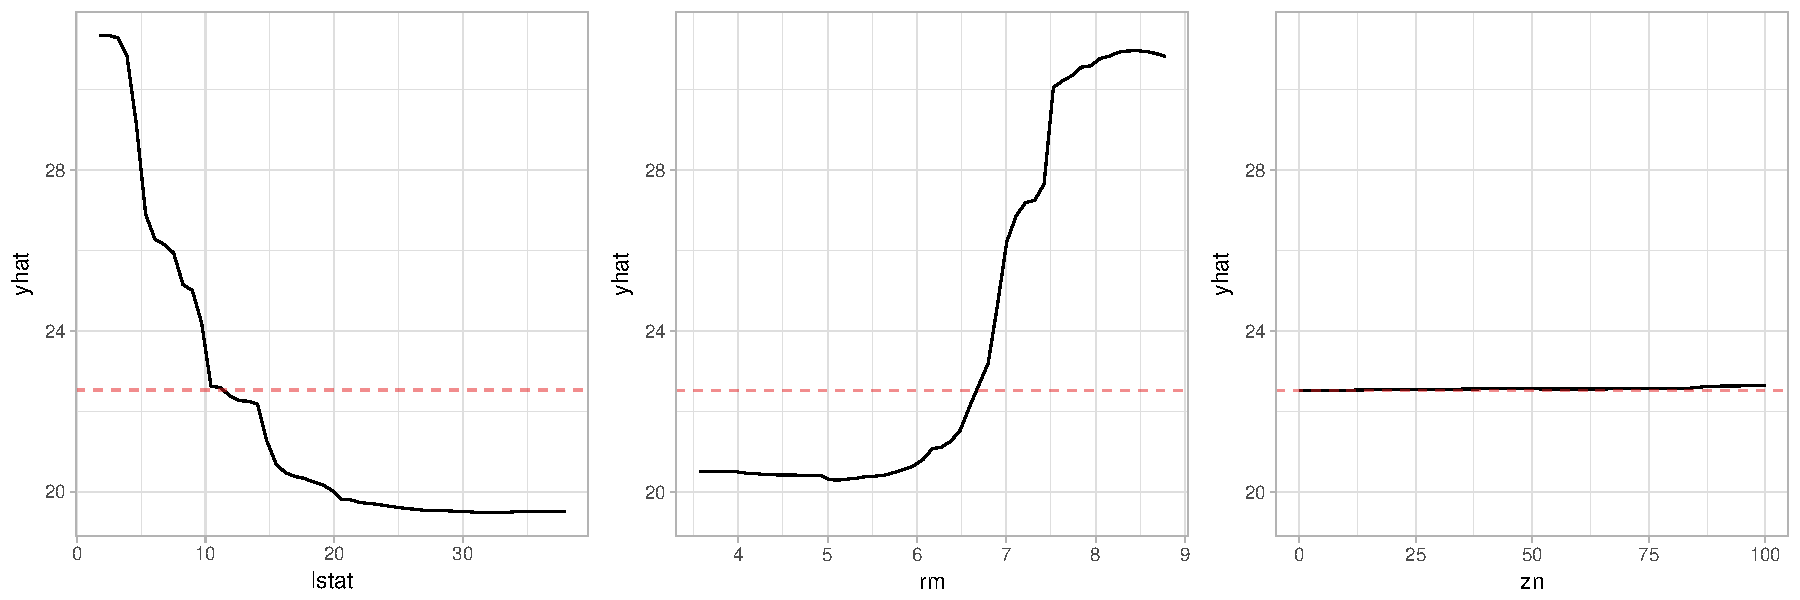
\includegraphics[width=1.0\textwidth]{boston-rf-pdps}
  \caption{TBD.}
\end{figure}


%%%%%%%%%%%%%%%%%%%%%%%%%%%%%%%%%%%%%%%%%%%%%%%%%%%%%%%%%%%%%%%%%%%%%%%%%%%%%%%%
% Examples
%%%%%%%%%%%%%%%%%%%%%%%%%%%%%%%%%%%%%%%%%%%%%%%%%%%%%%%%%%%%%%%%%%%%%%%%%%%%%%%%
\section{Examples: a simple function of ten variables}

For illustration, we use one of the regression problems described in Friedman (1991) and Breiman (1996). Inputs are 10 independent variables uniformly distributed on the interval $\left[0, 1\right]$; only 5 out of these 10 are actually used. Outputs are created according to the formula
\begin{equation}
\mathcal{Y} = 10 \sin\left(\pi x_1 x_2\right) + 20 \left(x_3 - 0.5\right) ^ 2 + 10 x_4 + 5 x_5 + \epsilon,
\end{equation}
where $\epsilon \sim \mathcal{N}\left(0, \sigma\right)$.


We fit a simple neural network with eight hidden units and a weight decay of 0.01. These parameters were chosen using 5-fold cross-validation to maximize the root mean squared error (RMSE). The network diagram is displayed in Figure~\ref{fig:network} below.
\begin{figure}[!htb]
  \label{network}
  \centering
  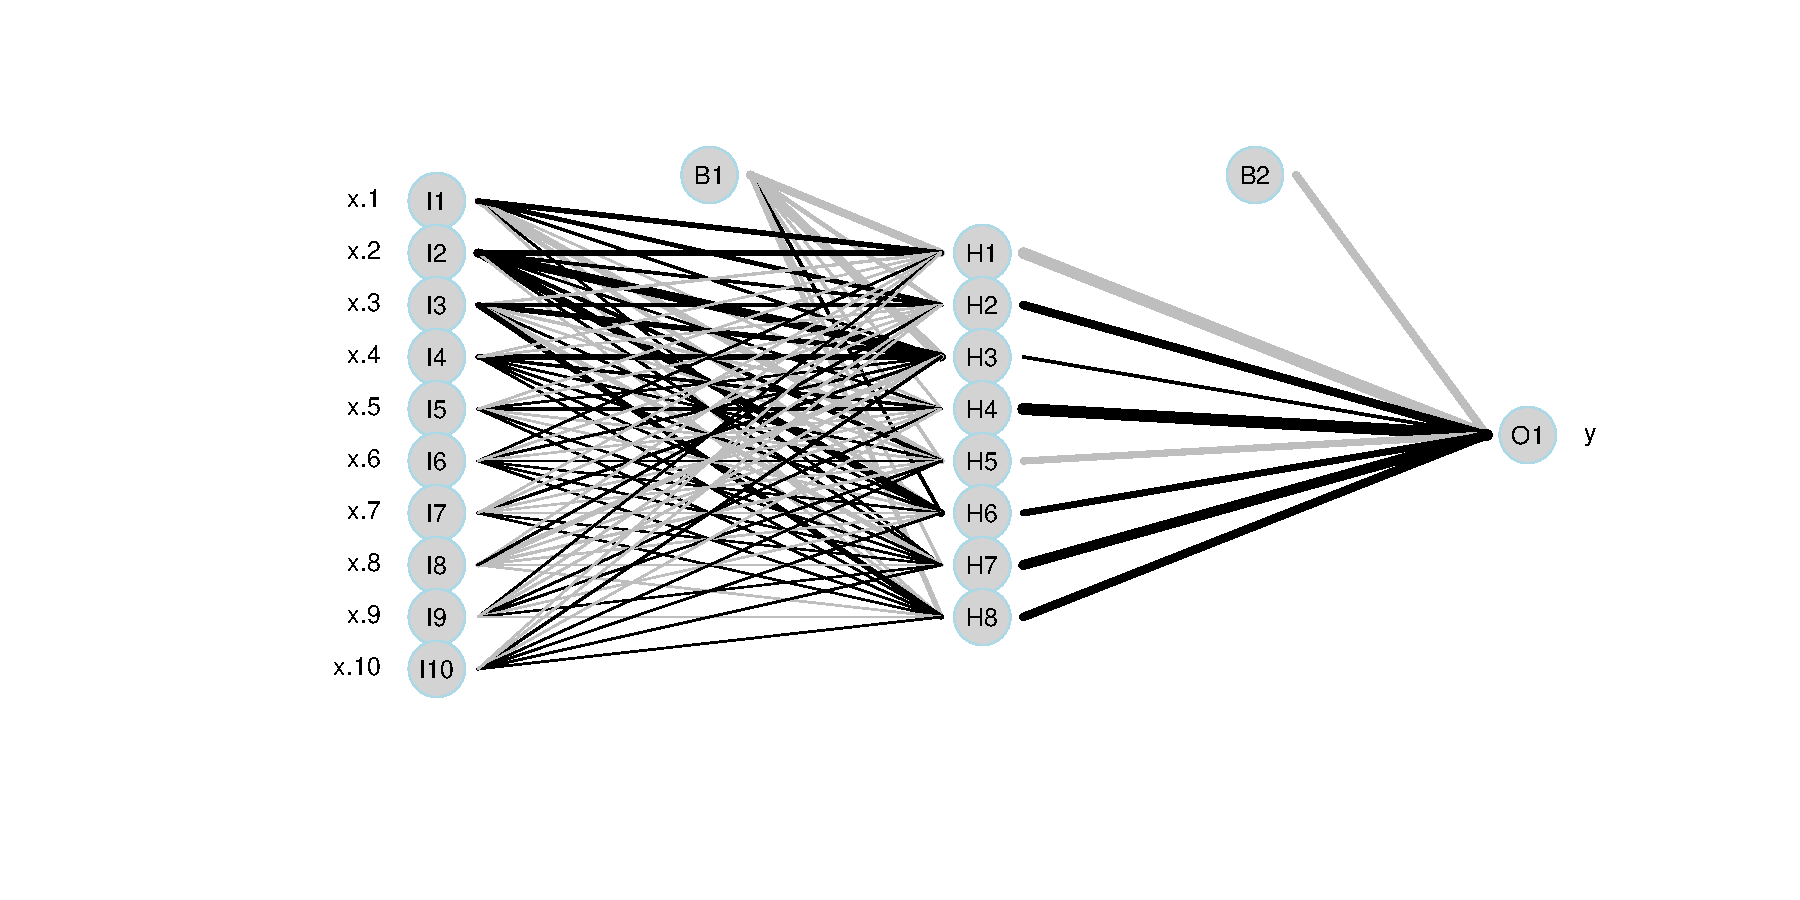
\includegraphics[width=1.0\textwidth]{network}
  \caption{Diagram of the neural network fitted to the Friedman 1 data set.}
\end{figure}

Variable importance plots are displayed in Figure~\ref{fig:network-vip}. Notice how the Garson and Olden algorithms incorrectly label some of the features not in the true model as "important".
\begin{figure}[!htb]
  \label{network-vip}
  \centering
  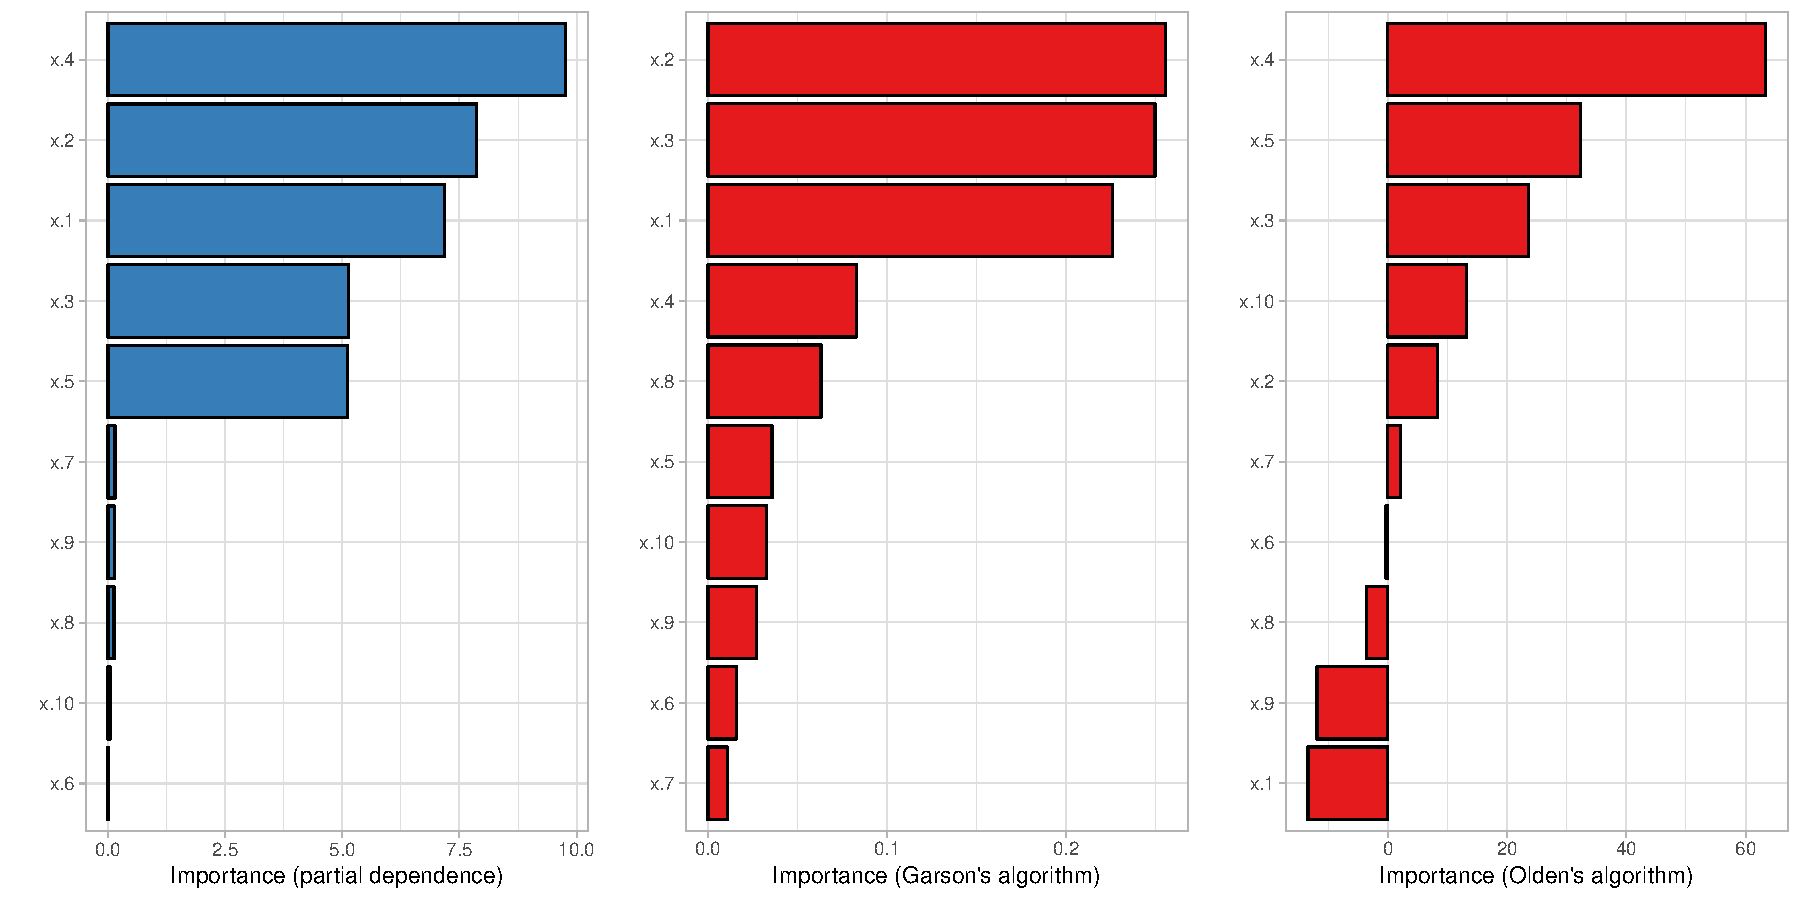
\includegraphics[width=1.0\textwidth]{network-vip}
  \caption{Variable importance plots for the neural network in Figure~\ref{fig:network}. \textit{Left}: partial dependence-based algorithm. \textit{Middle}: Garson's algorithm. \textit{Right}: Olden's algorithm.}
\end{figure}

For comparison, we fit a random forest [REFERENCE] with 1000 trees to the same data. Random forests (and other tree-based methods) have a natural way of denining variable importance. For details, see [REF]. Figure~\ref{fig:rf-vip} displays two types of importance measures obtained from the fitted random forest.


%%%%%%%%%%%%%%%%%%%%%%%%%%%%%%%%%%%%%%%%%%%%%%%%%%%%%%%%%%%%%%%%%%%%%%%%%%%%%%%%
% Discussion
%%%%%%%%%%%%%%%%%%%%%%%%%%%%%%%%%%%%%%%%%%%%%%%%%%%%%%%%%%%%%%%%%%%%%%%%%%%%%%%%
\section{Discussion}


%%%%%%%%%%%%%%%%%%%%%%%%%%%%%%%%%%%%%%%%%%%%%%%%%%%%%%%%%%%%%%%%%%%%%%%%%%%%%%%%
% Bibliography
%%%%%%%%%%%%%%%%%%%%%%%%%%%%%%%%%%%%%%%%%%%%%%%%%%%%%%%%%%%%%%%%%%%%%%%%%%%%%%%%
\bibliography{vip-methodology}

\end{document}
